\clearpage
\section{Stokes 方程的存在性与唯一性}
\label{sec:ch1-stokes-existence-uniqueness}

Stokes 方程是完整 Navier--Stokes 方程的线性化定常形式. 本节给出 Stokes 问题的变分表述, 利用投影定理证明存在性与唯一性, 并讨论无界区域情形以及解的正则性.

\subsection{问题的变分表述}
\label{subsec:ch1-stokes-variational-formulation}

设 $\Omega$ 是 $\mathbb R^n$ 中边界为 $\Gamma$ 的有界开集, $f\in\mathbf L^2(\Omega)$ 是 $\Omega$ 中给定的向量函数. 我们寻求表示流体速度的向量函数 $u=(u_1,\ldots,u_n)$ 和表示压力的标量函数 $p$, 它们定义在 $\Omega$ 中并满足下列方程与边界条件($\nu$ 是运动黏度系数, 为正常数):
\begin{equation}
-\nu\Delta u+\operatorname{grad}p=f\quad\text{在 }\Omega\text{ 中}\quad(\nu>0),
\label{eq:ch1-stokes-momentum}
\end{equation}
\begin{equation}
\operatorname{div}u=0\quad\text{在 }\Omega\text{ 中},
\label{eq:ch1-stokes-incompressibility}
\end{equation}
\begin{equation}
u=0\quad\text{在 }\Gamma\text{ 上}.
\label{eq:ch1-stokes-homogeneous-boundary}
\end{equation}
若 $f,u,p$ 是满足 \eqref{eq:ch1-stokes-momentum}--\eqref{eq:ch1-stokes-homogeneous-boundary} 的光滑函数, 则将 \eqref{eq:ch1-stokes-momentum} 与函数 $v\in\mathcal V$ 作标量积, 得
\[
(-\nu\Delta u+\operatorname{grad}p,v)=(f,v).
\]
\setcounter{footnote}{0}
分部积分后, 项 $(-\Delta u,v)$ 给出\footnote{参见 \ref{subsec:ch1-notation} 末尾的记号.}
\begin{equation}
\sum_{i=1}^n(\operatorname{grad}u_i,\operatorname{grad}v_i)=((u,v)),
\label{eq:ch1-stokes-gradient-form}
\end{equation}
而项 $(\operatorname{grad}p,v)$ 给出
\[
-(p,\operatorname{div}v)=0,
\]
从而得到
\begin{equation}
\nu((u,v))=(f,v),\qquad \forall v\in\mathcal V.
\label{eq:ch1-stokes-variational-smooth}
\end{equation}
由于 \eqref{eq:ch1-stokes-variational-smooth} 两边关于 $v$ 在线性意义下均依赖于 $H_0^1(\Omega)$ 拓扑且连续, 该等式通过连续性对 $\mathcal V$ 在 $H_0^1(\Omega)$ 中的闭包 $V$ 中每个 $v$ 仍成立. 若 $\Omega$ 是 $C^2$ 类集合, 则由 \eqref{eq:ch1-stokes-homogeneous-boundary}, 光滑函数 $u$ 属于 $\mathbf H_0^1(\Omega)$; 又由 \eqref{eq:ch1-stokes-incompressibility} 和定理 \ref{thm:ch1-characterization-v}, 有 $u\in V$. 因而得到结论:
\begin{equation}
u\in V,\qquad \nu((u,v))=(f,v),\quad\forall v\in V.
\label{eq:ch1-stokes-variational-problem}
\end{equation}

反过来, 假设 $u$ 满足 \eqref{eq:ch1-stokes-variational-problem}, 我们说明 $u$ 在某种意义下满足 \eqref{eq:ch1-stokes-momentum}--\eqref{eq:ch1-stokes-homogeneous-boundary}. 因为 $u$ 仅属于 $\mathbf H_0^1(\Omega)$, 其正则性低于上述情形, 所以只能期望这些方程以弱于经典意义的方式成立. 实际上, $u\in\mathbf H_0^1(\Omega)$ 意味着其各分量的迹 $\gamma_0u$ 在 $\mathbf H^{1/2}(\Gamma)$ 中为零; $u\in V$ 结合定理 \ref{thm:ch1-characterization-v} 意味着 $\operatorname{div}u=0$ 在分布意义下成立; 由 \eqref{eq:ch1-stokes-variational-problem} 又有
\[
\langle-\nu\Delta u-f,v\rangle=0,\qquad\forall v\in\mathcal V.
\]
因此, 由命题 \ref{prop:ch1-de-rham-gradient} 和命题 \ref{prop:ch1-gradient-regularity}, 存在某个分布 $p\in L^2(\Omega)$, 使
\[
\nu\Delta u-f=-\operatorname{grad}p
\]
在 $\Omega$ 中以分布意义成立. 我们由此证明了下述引理.

\MBSourceStatementNumber{lemma}{1}
\begin{Lemma}
\label{lem:ch1-stokes-variational-equivalence}
设 $\Omega$ 是 $C^2$ 类有界开集. 下列条件等价:

(i) $u\in V$ 满足 \eqref{eq:ch1-stokes-variational-problem}.

(ii) $u\in\mathbf H_0^1(\Omega)$, 并在下述弱意义下满足 \eqref{eq:ch1-stokes-momentum}--\eqref{eq:ch1-stokes-homogeneous-boundary}:
\begin{equation}
\text{存在 }p\in L^2(\Omega),\text{ 使 }-\nu\Delta u+\operatorname{grad}p=f
\quad\text{在 }\Omega\text{ 中以分布意义成立};
\label{eq:ch1-stokes-weak-momentum}
\end{equation}
\begin{equation}
\operatorname{div}u=0\quad\text{在 }\Omega\text{ 中以分布意义成立};
\label{eq:ch1-stokes-weak-incompressibility}
\end{equation}
\begin{equation}
\gamma_0u=0.
\label{eq:ch1-stokes-weak-boundary}
\end{equation}
\end{Lemma}

\MBSourceStatementNumber{definition}{1}
\begin{Definition}
\label{def:ch1-stokes-variational-formulation}
问题``求满足 \eqref{eq:ch1-stokes-variational-problem} 的 $u\in V$''称为问题 \eqref{eq:ch1-stokes-momentum}--\eqref{eq:ch1-stokes-homogeneous-boundary} 的变分表述.
\end{Definition}

\MBSourceStatementNumber{remark}{1}
\begin{Remark}
\label{rem:ch1-stokes-variational-observations}
在研究 \eqref{eq:ch1-stokes-variational-problem} 的存在性与唯一性之前, 先作几点说明.

(i) 问题 \eqref{eq:ch1-stokes-momentum}--\eqref{eq:ch1-stokes-homogeneous-boundary} 的变分表述由 J. Leray [1, 2, 3] 引入. 它把经典问题化为仅求 $u$ 的问题; $p$ 的存在性随后由命题 \ref{prop:ch1-de-rham-gradient} 推出.

(ii) 当 $\Omega$ 不光滑或无界时, 在定理 \ref{thm:ch1-characterization-v} 的证明中出现了两个可能不同的空间 $V$ 和 $V^\bullet$(有 $V\subset V^\bullet$; 参见注 \ref{rem:ch1-v-star-shaped} (ii)):
\[
V=\mathcal V\text{ 在 }\mathbf H_0^1(\Omega)\text{ 中的闭包},
\qquad
V^\bullet=\{u\in\mathbf H_0^1(\Omega):\operatorname{div}u=0\}.
\]
于是可提出两个可能不同的变分问题: 一个恰为 \eqref{eq:ch1-stokes-variational-problem}, 另一个则把其中的 $V$ 换成 $V^\bullet$. 一般情形下, $V$ 与 $V^\bullet$ 的关系以及这两个变分问题之间的关系均未知. J.G. Heywood [2] 研究了这些问题之间的关系; O.A. Ladyzhenskaya--V.A. Solonnikov [1] 则研究了上述作者所考虑的情形(注 \ref{rem:ch1-v-star-shaped} (ii)).

出于技术原因, 特别是在非线性情形下极为重要的原因, 我们总是在空间 $V$ 中工作, 并且只考虑变分问题 \eqref{eq:ch1-stokes-variational-problem}.

作为引理 \ref{lem:ch1-stokes-variational-equivalence} 的补充, 对任意集合 $\Omega$, 若 $u$ 满足 \eqref{eq:ch1-stokes-variational-problem}(或其中以 $V^\bullet$ 代替 $V$), 则它满足 \eqref{eq:ch1-stokes-weak-momentum}, 但只能保证 $p\in L^2_{\mathrm{loc}}(\Omega)$; 它不加修改地满足 \eqref{eq:ch1-stokes-weak-incompressibility}; 它还在 $u\in\mathbf H_0^1(\Omega)$ 的意义下满足 \eqref{eq:ch1-stokes-weak-boundary}, 更精确的含义取决于 $\Omega$ 上可用的迹定理.
\end{Remark}

\subsection{投影定理}
\label{subsec:ch1-projection-theorem}

设 $\Omega$ 是 $\mathbb R^n$ 中任意开集, 且
\begin{equation}
\Omega\text{ 在某个方向上有界}.
\label{eq:ch1-domain-bounded-one-direction}
\end{equation}
根据 \eqref{eq:ch1-h01-gradient-norm}, $H_0^1(\Omega)$ 对标量积 \eqref{eq:ch1-stokes-gradient-form} 是 Hilbert 空间; $\mathcal V$ 由 \eqref{eq:ch1-test-divergence-free-space} 定义, $V$ 是 $\mathcal V$ 在 $\mathbf H_0^1(\Omega)$ 中的闭包.

\MBSourceStatementNumber{theorem}{1}
\begin{Theorem}
\label{thm:ch1-stokes-existence-uniqueness}
设开集 $\Omega\subset\mathbb R^n$ 在某个方向上有界. 对每个 $f\in\mathbf L^2(\Omega)$, 问题 \eqref{eq:ch1-stokes-variational-problem} 有唯一解 $u$.(当 $f\in\mathbf H^{-1}(\Omega)$ 时, 结论仍成立.)

此外, 存在函数 $p\in L^2_{\mathrm{loc}}(\Omega)$, 使 \eqref{eq:ch1-stokes-weak-momentum}--\eqref{eq:ch1-stokes-weak-incompressibility} 成立.

若 $\Omega$ 是 $C^2$ 类有界开集, 则 $p\in L^2(\Omega)$, 且 $u,p$ 满足 \eqref{eq:ch1-stokes-weak-momentum}--\eqref{eq:ch1-stokes-weak-boundary}.
\end{Theorem}

这个定理是前述引理和下面经典投影定理的直接推论.

\MBSourceStatementNumber{theorem}{2}
\begin{Theorem}
\label{thm:ch1-abstract-projection}
设 $W$ 是可分实 Hilbert 空间, 范数为 $\lVert\cdot\rVert_W$, $a(u,v)$ 是 $W\times W$ 上连续双线性形式, 且它是强制的, 即存在 $\alpha>0$, 使
\begin{equation}
a(u,u)\geq\alpha\lVert u\rVert_W^2,\qquad\forall u\in W.
\label{eq:ch1-coercivity}
\end{equation}
则对 $W$ 的对偶空间 $W'$ 中每个 $\ell$, 存在唯一的 $u\in W$, 使
\begin{equation}
a(u,v)=\langle\ell,v\rangle,\qquad\forall v\in W.
\label{eq:ch1-abstract-variational-problem}
\end{equation}
\end{Theorem}

为了把该定理应用于 \eqref{eq:ch1-stokes-variational-problem}, 取 $W=V$, 并赋予它由 \eqref{eq:ch1-stokes-gradient-form} 决定的范数; 令 $a(u,v)=\nu((u,v))$, 并令 $v\mapsto\langle\ell,v\rangle$ 为 $v\mapsto(f,v)$, 这显然是 $V$ 上的连续线性形式. 空间 $V$ 是可分空间 $\mathbf H_0^1(\Omega)$ 的闭子空间, 因而可分.

\begin{Proof}
先证定理 \ref{thm:ch1-abstract-projection} 的唯一性. 设 $u_1,u_2$ 是 \eqref{eq:ch1-abstract-variational-problem} 的两个解, 令 $u=u_1-u_2$. 则
\[
a(u_1,v)=a(u_2,v)=\langle\ell,v\rangle,\qquad\forall v\in W,
\]
\[
a(u_1-u_2,v)=0,\qquad\forall v\in W.
\]
在后一等式中取 $v=u$, 由 \eqref{eq:ch1-coercivity} 得
\[
\alpha\lVert u\rVert_W^2\leq a(u,u)=0,
\]
故 $u=0$.

再证存在性. 由于 $W$ 可分, 存在 $W$ 中一个自由且完备的序列 $w_1,\ldots,w_m,\ldots$. 令 $W_m$ 为 $w_1,\ldots,w_m$ 张成的空间. 对每个固定的整数 $m$, 在 $W_m$ 中定义 \eqref{eq:ch1-abstract-variational-problem} 的近似解, 即向量 $u_m\in W_m$,
\begin{equation}
u_m=\sum_{i=1}^m\xi_{i,m}w_i,\qquad\xi_{i,m}\in\mathbb R,
\label{eq:ch1-galerkin-approximation}
\end{equation}
满足
\begin{equation}
a(u_m,v)=\langle\ell,v\rangle,\qquad\forall v\in W_m.
\label{eq:ch1-galerkin-equations}
\end{equation}
我们说明存在唯一的 $u_m$ 满足 \eqref{eq:ch1-galerkin-equations}. 该式等价于 $m$ 个方程
\begin{equation}
a(u_m,w_j)=\langle\ell,w_j\rangle,\qquad j=1,\ldots,m,
\label{eq:ch1-galerkin-basis-equations}
\end{equation}
也等价于关于 $u_m$ 的 $m$ 个分量 $\xi_{i,m}$ 的线性方程组
\begin{equation}
\sum_{i=1}^m\xi_{i,m}a(w_i,w_j)=\langle\ell,w_j\rangle,
\qquad j=1,\ldots,m.
\label{eq:ch1-galerkin-linear-system}
\end{equation}
$u_m$ 的存在性与唯一性只须由这个线性方程组的正则性推出. 为此只须证明其对应的齐次方程组
\begin{equation}
\sum_{i=2}^m\xi_i a(w_i,w_j)=0,\qquad j=1,\ldots,m,
\label{eq:ch1-galerkin-homogeneous-system}
\end{equation}
只有解 $\xi_1=\cdots=\xi_m=0$. 若 $\xi_1,\ldots,\xi_m$ 满足 \eqref{eq:ch1-galerkin-homogeneous-system}, 将各方程分别乘以相应的 $\xi_j$ 后相加, 得
\[
\sum_{i,j=1}^m\xi_i\xi_j a(w_i,w_j)=0,
\]
或由 $a$ 的双线性性,
\[
a\left(\sum_{i=1}^m\xi_iw_i,\sum_{j=1}^m\xi_jw_j\right)=0.
\]
利用 \eqref{eq:ch1-coercivity} 得
\[
\sum_{i=1}^m\xi_iw_i=0,
\]
最终由 $w_1,\ldots,w_m$ 线性无关得到 $\xi_1=\cdots=\xi_m=0$.

下面传递到极限. 在 \eqref{eq:ch1-galerkin-equations} 中取 $v=u_m$, 得
\begin{equation}
a(u_m,u_m)=\langle\ell,u_m\rangle.
\label{eq:ch1-galerkin-energy-identity}
\end{equation}
由 \eqref{eq:ch1-coercivity},
\[
\alpha\lVert u_m\rVert_W^2\leq a(u_m,u_m)
=\langle\ell,u_m\rangle
\leq\lVert\ell\rVert_{W'}\lVert u_m\rVert_W,
\]
故
\begin{equation}
\lVert u_m\rVert_W\leq\frac1\alpha\lVert\ell\rVert_{W'}.
\label{eq:ch1-galerkin-uniform-bound}
\end{equation}
这证明序列 $u_m$ 在 $W$ 中关于 $m$ 一致有界. Hilbert 空间中的闭球弱紧, 因而存在 $u\in W$ 以及从 $u_m$ 中抽取的子序列 $u_{m'}$, $m'\to\infty$, 使
\begin{equation}
u_{m'}\rightharpoonup u\quad\text{在 }W\text{ 的弱拓扑中},\qquad m'\to\infty.
\label{eq:ch1-galerkin-weak-convergence}
\end{equation}
固定 $v\in W_j$. 当 $m'\geq j$ 时, $v\in W_{m'}$, 由 \eqref{eq:ch1-galerkin-equations},
\[
a(u_{m'},v)=\langle\ell,v\rangle.
\]
利用下述引理, 可令 $m'\to\infty$, 得
\begin{equation}
a(u,v)=\langle\ell,v\rangle.
\label{eq:ch1-galerkin-limit-equation}
\end{equation}
等式 \eqref{eq:ch1-galerkin-limit-equation} 对每个 $v\in\bigcup_{j=1}^{\infty}W_j$ 成立; 该集合在 $W$ 中稠密, 所以由连续性, 该等式对所有 $v\in W$ 仍成立. 因而 $u$ 是 \eqref{eq:ch1-abstract-variational-problem} 的解.
\end{Proof}

\MBSourceStatementNumber{lemma}{2}
\begin{Lemma}
\label{lem:ch1-bilinear-weak-strong-limits}
设 $a(u,v)$ 是 Hilbert 空间 $W$ 上的连续双线性形式. 设 $\phi_m$(或 $\psi_m$) 是 $W$ 中依弱拓扑(或强拓扑)收敛到 $\phi$(或 $\psi$)的序列. 则
\begin{equation}
\lim_{m\to\infty}a(\psi_m,\phi_m)=a(\psi,\phi),
\label{eq:ch1-bilinear-strong-weak-limit}
\end{equation}
\begin{equation}
\lim_{m\to\infty}a(\phi_m,\psi_m)=a(\phi,\psi).
\label{eq:ch1-bilinear-weak-strong-limit}
\end{equation}
\end{Lemma}

\begin{Proof}
写成
\[
a(\psi_m,\phi_m)-a(\psi,\phi)
=a(\psi_m-\psi,\phi_m)+a(\psi,\phi_m-\phi).
\]
由于 $a$ 连续且序列 $\phi_m$ 有界,
\[
|a(\psi_m-\psi,\phi_m)|
\leq c\lVert\psi_m-\psi\rVert_W\lVert\phi_m\rVert_W
\leq c'\lVert\psi_m-\psi\rVert_W,
\]
当 $m\to\infty$ 时此项趋于 $0$.

再注意线性算子 $v\mapsto a(\psi,v)$ 在 $W$ 上连续, 故存在 $W'$ 中某个依赖于 $\psi$ 的元素 $A(\psi)$, 使
\begin{equation}
a(\psi,v)=\langle A(\psi),v\rangle,\qquad\forall v\in W.
\label{eq:ch1-bilinear-associated-operator}
\end{equation}
于是
\[
a(\psi,\phi_m-\phi)=\langle A(\psi),\phi_m-\phi\rangle,
\]
由 $\phi_m$ 的弱收敛, 当 $m\to\infty$ 时该式趋于 $0$. 这证明了 \eqref{eq:ch1-bilinear-strong-weak-limit}. 对双线性形式
\[
a^*(u,v)=a(v,u)
\]
应用 \eqref{eq:ch1-bilinear-strong-weak-limit}, 即得 \eqref{eq:ch1-bilinear-weak-strong-limit}.
\end{Proof}

\MBSourceStatementNumber{remark}{2}
\begin{Remark}
\label{rem:ch1-projection-theorem-comments}
(i) 当 $f\in\mathbf H^{-1}(\Omega)$ 时, 定理 \ref{thm:ch1-stokes-existence-uniqueness} 仍成立.

(ii) 可以证明, 定理 \ref{thm:ch1-abstract-projection} 的证明中构造的整个序列 $\{u_m\}$ 在 $W$ 的强拓扑中收敛到 \eqref{eq:ch1-abstract-variational-problem} 的解 $u$. 此处不证明这一结果; 它将作为 \MBUnresolvedReference{theorem}{3.1} 的推论出现.

(iii) 利用引理 \ref{lem:ch1-bilinear-weak-strong-limits} 证明中引入的 $A(\psi)$(参见 \eqref{eq:ch1-bilinear-associated-operator}), 可将 \eqref{eq:ch1-abstract-variational-problem} 写为
\[
\langle A(u),v\rangle=\langle\ell,v\rangle,
\]
这等价于
\begin{equation}
A(u)=\ell\quad\text{在 }W'\text{ 中}.
\label{eq:ch1-operator-equation}
\end{equation}
投影定理的另一种经典证明是说明算子 $u\mapsto A(u)$ 是 $W$ 到 $W'$ 的同构; 参见 R. Temam [8].
\end{Remark}

\subsubsection*{一个变分性质}

\MBSourceStatementNumber{proposition}{1}
\begin{Proposition}
\label{prop:ch1-stokes-energy-minimizer}
\eqref{eq:ch1-stokes-variational-problem} 的解 $u$ 也是 $V$ 中唯一满足
\begin{equation}
E(u)\leq E(v),\qquad\forall v\in V,
\label{eq:ch1-stokes-energy-minimum}
\end{equation}
的元素, 其中
\begin{equation}
E(v)=\nu\lVert v\rVert^2-2(f,v).
\label{eq:ch1-stokes-energy-functional}
\end{equation}
\end{Proposition}

\begin{Proof}
设 $u$ 是 \eqref{eq:ch1-stokes-variational-problem} 的解. 由于
\[
\lVert u-v\rVert^2\geq0,\qquad\forall v\in V,
\]
有
\begin{equation}
\nu\lVert u\rVert^2+\nu\lVert v\rVert^2-2\nu((u,v))\geq0.
\label{eq:ch1-stokes-energy-expansion}
\end{equation}
由 \eqref{eq:ch1-stokes-variational-problem},
\[
-\nu\lVert u\rVert^2
=\nu\lVert u\rVert^2-2(f,u)=E(u),
\qquad
-2\nu((u,v))=-2(f,v),
\]
故 \eqref{eq:ch1-stokes-energy-expansion} 恰好给出 \eqref{eq:ch1-stokes-energy-minimum}.

反之, 若 $u\in V$ 满足 \eqref{eq:ch1-stokes-energy-minimum}, 则对任意 $v\in V$ 和 $\lambda\in\mathbb R$,
\[
E(u)\leq E(u+\lambda v).
\]
这可化为
\begin{equation}
\nu\lambda^2\lVert v\rVert^2
+2\lambda\nu((u,v))-2\lambda(f,v)\geq0,
\qquad\forall\lambda\in\mathbb R.
\label{eq:ch1-stokes-energy-quadratic}
\end{equation}
该不等式对每个 $\lambda\in\mathbb R$ 成立, 只有当
\[
\nu((u,v))=(f,v)
\]
时才可能. 因此 $u$ 确为 \eqref{eq:ch1-stokes-variational-problem} 的解.
\end{Proof}

\MBSourceStatementNumber{remark}{3}
\begin{Remark}
\label{rem:ch1-stokes-vbullet-problem}
若注 \ref{rem:ch1-stokes-variational-observations} 中的空间 $V$ 与 $V^\bullet$ 不同, 定理 \ref{thm:ch1-abstract-projection} 仍给出唯一的 $\widetilde u\in V^\bullet$, 使
\begin{equation}
\nu((\widetilde u,v))=(f,v),\qquad\forall v\in V^\bullet.
\label{eq:ch1-stokes-vbullet-variational}
\end{equation}
命题 \ref{prop:ch1-stokes-energy-minimizer} 中的 $u,V$ 也可分别换成 $\widetilde u,V^\bullet$.
\end{Remark}
\subsection{无界情形}
\label{subsec:ch1-stokes-unbounded-domain}

这里考虑 $\Omega$ 无界且不满足 \eqref{eq:ch1-domain-bounded-one-direction} 的情形. 若 $\Omega$ 是 $C^2$ 类集合, 问题 \eqref{eq:ch1-stokes-momentum}--\eqref{eq:ch1-stokes-homogeneous-boundary} 不再像引理 \ref{lem:ch1-stokes-variational-equivalence} 中那样与 \eqref{eq:ch1-stokes-variational-problem} 等价. 原因在于: 若 $u$ 是 \eqref{eq:ch1-stokes-momentum}--\eqref{eq:ch1-stokes-homogeneous-boundary} 的经典解, 在没有关于 $u$ 在无穷远处行为的进一步信息时, 不能断定 $u\in\mathbf H_0^1(\Omega)$; 因而可能有 $u\notin V$, 且等式 \eqref{eq:ch1-stokes-variational-smooth} 不能通过连续性延拓到 $\mathcal V$ 的闭包 $V$. 直接利用定理 \ref{thm:ch1-abstract-projection} 求解 \eqref{eq:ch1-stokes-variational-problem} 也有困难: 假设 \eqref{eq:ch1-coercivity} 不成立, $V$ 对范数
\[
[[u]]=\sqrt{|u|^2+\lVert u\rVert^2}
\]
是 Hilbert 空间, 但由于失去了 Poincaré 不等式, 该范数与范数 $\lVert u\rVert$ 不等价.

为了在一般情形下提出并求解变分问题, 引入空间
\begin{equation}
Y=\mathcal V\text{ 关于范数 }\lVert\cdot\rVert\text{ 的完备化}.
\label{eq:ch1-y-space-definition}
\end{equation}
由于 $\lVert u\rVert\leq[[u]]$, 显然 $Y$ 比 $V$ 更大:
\begin{equation}
V\subset Y.
\label{eq:ch1-v-in-y}
\end{equation}

\MBSourceStatementNumber{lemma}{3}
\begin{Lemma}
\label{lem:ch1-y-space-embeddings}
若 $n\geq3$, 则
\begin{equation}
Y\subset\{u\in\mathbf L^\alpha(\Omega):D_i u\in\mathbf L^2(\Omega),\ 1\leq i\leq n\},
\label{eq:ch1-y-embedding-high-dimensional}
\end{equation}
其中 $\alpha=2n/(n-2)$. 若 $n=2$, 则
\begin{equation}
Y\subset\{u\in\mathbf L^\alpha_{\mathrm{loc}}(\Omega):D_i u\in\mathbf L^2(\Omega),\ i=1,2\},
\qquad\forall\alpha\geq1.
\label{eq:ch1-y-embedding-two-dimensional}
\end{equation}
这些嵌入连续.
\end{Lemma}

\begin{Proof}
先证明 \eqref{eq:ch1-y-embedding-high-dimensional}. 它是 Sobolev 不等式的推论(见 Sobolev [1], Lions [1] 以及 \MBUnresolvedReference{chapter}{2}):
\begin{equation}
\lVert\phi\rVert_{L^\alpha(\Omega)}
\leq c(\alpha,n)\lVert\operatorname{grad}\phi\rVert_{\mathbf L^2(\Omega)},
\qquad\forall\phi\in\mathcal D(\Omega),
\label{eq:ch1-sobolev-inequality-unbounded}
\end{equation}
其中 $\alpha=2m/(n-2)$.

若 $u\in Y$, 则存在 $u_m\in\mathcal V$ 在 $Y$ 中收敛到 $u$; 由 \eqref{eq:ch1-sobolev-inequality-unbounded},
\[
\lVert u_m-u_p\rVert_{\mathbf L^\alpha(\Omega)}
\leq c'(\alpha,n)\lVert u_m-u_p\rVert,
\]
\begin{equation}
\lVert u_m-u_p\rVert_Z\leq c''\lVert u_m-u_p\rVert,
\label{eq:ch1-y-cauchy-estimate}
\end{equation}
其中 $Z$ 表示包含关系 \eqref{eq:ch1-y-embedding-high-dimensional} 右端的空间, $\lVert\cdot\rVert_Z$ 是 $Z$ 的自然范数:
\[
\lVert u\rVert_Z=\lVert u\rVert_{\mathbf L^\alpha(\Omega)}+\lVert u\rVert.
\]
当 $m,p$ 趋于无穷时, \eqref{eq:ch1-y-cauchy-estimate} 右端趋于 $0$. 因而 $u_m$ 是 $Z$ 中的 Cauchy 序列, 其极限 $u$ 属于 $Z$. 显然还有
\[
\lVert u\rVert_Z\leq c''\lVert u\rVert,
\]
其中 $c''$ 与 \eqref{eq:ch1-y-cauchy-estimate} 中相同($c''=c''(n)$).

对 \eqref{eq:ch1-y-embedding-two-dimensional} 的证明类似, 只须在 $\Omega'$ 是 $\Omega$ 的紧子集时考虑 $L^\alpha(\Omega')$ 中的 Cauchy 序列.
\end{Proof}

\MBSourceStatementNumber{theorem}{3}
\begin{Theorem}
\label{thm:ch1-stokes-unbounded-existence}
设 $\Omega$ 是 $\mathbb R^n$ 中任意开集, $f\in Y'$, 其中 $Y'$ 是 \eqref{eq:ch1-y-space-definition} 中空间 $Y$ 的对偶. 则存在唯一的 $u\in Y$, 使
\begin{equation}
\nu((u,v))=\langle f,v\rangle,
\qquad\forall v\in Y.
\label{eq:ch1-stokes-unbounded-variational}
\end{equation}
存在 $p\in L^2_{\mathrm{loc}}(\Omega)$, 使 \eqref{eq:ch1-stokes-weak-momentum} 成立, 且 \eqref{eq:ch1-stokes-weak-incompressibility} 为真.
\end{Theorem}

\begin{Proof}
将定理 \ref{thm:ch1-abstract-projection} 应用于空间 $Y$, 取 $a(u,v)=\nu((u,v))$, 并以 $f$ 代替 $\ell$, 得到满足 \eqref{eq:ch1-stokes-unbounded-variational} 的唯一 $u$.

于是注 \ref{rem:ch1-gradient-operator-range} (i) 表明, 存在 $p\in L^2_{\mathrm{loc}}(\Omega)$, 使 \eqref{eq:ch1-stokes-weak-momentum} 成立; \eqref{eq:ch1-stokes-weak-incompressibility} 自然容易验证. 最后, \eqref{eq:ch1-stokes-weak-boundary} 在某种意义下成立, 其含义取决于 $Y$(或包含关系 \eqref{eq:ch1-y-embedding-high-dimensional} 和 \eqref{eq:ch1-y-embedding-two-dimensional} 右端的空间 $Z$)可用的迹定理.

若 $\Omega$ 局部 Lipschitz, 则命题 \ref{prop:ch1-gradient-regularity} 表明 $p\in L^2_{\mathrm{loc}}(\overline\Omega)$.
\end{Proof}

\MBSourceStatementNumber{remark}{4}
\begin{Remark}
\label{rem:ch1-stokes-unbounded-data}
由引理 \ref{lem:ch1-y-space-embeddings}, 对 $f\in\mathbf L^{\alpha'}(\Omega)$, 其中 $1/\alpha+1/\alpha'=1$, 映射
\begin{equation}
v\longmapsto\int_\Omega f\cdot v\,dx
\label{eq:ch1-y-dual-integral}
\end{equation}
是 $Y$ 上的连续线性形式. 因而在定理 \ref{thm:ch1-stokes-unbounded-existence} 中可取任意 $f\in\mathbf L^{\alpha'}(\Omega)$, 其中 $\alpha=2n/(n-2)$, $n\geq3$.
\end{Remark}

\subsection{非齐次 Stokes 问题}
\label{subsec:ch1-nonhomogeneous-stokes}

下面考虑非齐次 Stokes 问题.

\MBSourceStatementNumber{theorem}{4}
\begin{Theorem}
\label{thm:ch1-nonhomogeneous-stokes}
设 $\Omega$ 是 $\mathbb R^n$ 中 $C^2$ 类有界开集. 给定
\[
f\in\mathbf H^{-1}(\Omega),\qquad g\in L^2(\Omega),\qquad
\phi\in\mathbf H^{1/2}(\Gamma),
\]
并且
\begin{equation}
\int_\Omega g\,dx=\int_\Gamma\phi\cdot\nu\,d\Gamma.
\label{eq:ch1-nonhomogeneous-compatibility}
\end{equation}
则存在
\[
u\in\mathbf H^1(\Omega),\qquad p\in L^2(\Omega),
\]
它们是非齐次 Stokes 问题
\begin{equation}
-\nu\Delta u+\operatorname{grad}p=f\quad\text{在 }\Omega\text{ 中},
\label{eq:ch1-nonhomogeneous-momentum}
\end{equation}
\begin{equation}
\operatorname{div}u=g\quad\text{在 }\Omega\text{ 中},
\label{eq:ch1-nonhomogeneous-divergence}
\end{equation}
\begin{equation}
\gamma_0u=\phi,\quad\text{即 }u=\phi\quad\text{在 }\Gamma\text{ 上}
\label{eq:ch1-nonhomogeneous-boundary}
\end{equation}
的解. $u$ 唯一, $p$ 在相差一个加性常数的意义下唯一.
\end{Theorem}

\begin{Proof}
因为 $\mathbf H^{1/2}(\Gamma)=\gamma_0\mathbf H^1(\Omega)$, 存在 $u_0\in\mathbf H^1(\Omega)$, 使 $\gamma_0u_0=\phi$. 由 \eqref{eq:ch1-nonhomogeneous-compatibility} 和 Stokes 公式,
\[
\int_\Omega(g-\operatorname{div}u_0)\,dx=0.
\]
利用下述引理可知, 存在 $u_1\in\mathbf H_0^1(\Omega)$, 使
\[
\operatorname{div}u_1=g-\operatorname{div}u_0.
\]
令 $v=u-u_0-u_1$, 问题 \eqref{eq:ch1-nonhomogeneous-momentum}--\eqref{eq:ch1-nonhomogeneous-boundary} 化为关于 $v$ 的齐次 Stokes 问题:
\[
-\nu\Delta v+\operatorname{grad}p
=f-\nu\Delta(u_0+u_1)\in\mathbf H^{-1}(\Omega),
\]
\[
\operatorname{div}v=0\quad\text{在 }\Omega\text{ 中},
\qquad
v=0\quad\text{在 }\partial\Omega\text{ 上}.
\]
由此得到 $v,p$ 的存在性与唯一性, 进而得到 $u,p$ 的存在性与唯一性.
\end{Proof}

\MBSourceStatementNumber{lemma}{4}
\begin{Lemma}
\label{lem:ch1-divergence-surjective}
设 $\Omega$ 是 $\mathbb R^n$ 中 Lipschitz 有界开集. 则散度算子把 $\mathbf H_0^1(\Omega)$ 映满空间 $L^2(\Omega)/\mathbb R$, 即
\begin{equation}
\left\{g\in L^2(\Omega):\int_\Omega g(x)\,dx=0\right\}.
\label{eq:ch1-zero-mean-l2-space}
\end{equation}
\end{Lemma}

\begin{Proof}
由命题 \ref{prop:ch1-gradient-regularity} 和注 \ref{rem:ch1-gradient-operator-range} (ii), $A=\operatorname{grad}$ 是从 $L^2(\Omega)$ 到 $\mathbf H^{-1}(\Omega)$ 的连续线性算子, 并且是 \eqref{eq:ch1-zero-mean-l2-space} 到其值域 $R(A)$ 的同构. 通过转置, 其伴随算子
\[
A^*=-\operatorname{div}\in\mathcal L(\mathbf H_0^1(\Omega),L^2(\Omega))
\]
是从 $R(A)$ 的正交补到空间 \eqref{eq:ch1-zero-mean-l2-space} 的同构; 特别地, $A^*$ 把 $\mathbf H_0^1(\Omega)$ 映满 $L^2(\Omega)/\mathbb R$.
\end{Proof}

\MBSourceStatementNumber{remark}{5}
\begin{Remark}
\label{rem:ch1-nonhomogeneous-lipschitz-extension}
定理 \ref{thm:ch1-nonhomogeneous-stokes} 易于推广到 $\Omega$ 仅为 $\mathbb R^n$ 中 Lipschitz 有界开集的情形, 只须把 $\phi$ 给成某个 $\phi_0\in\mathbf H^1(\Omega)$ 的迹, 并把 \eqref{eq:ch1-nonhomogeneous-compatibility} 和 \eqref{eq:ch1-nonhomogeneous-boundary} 分别理解为
\begin{equation*}
\tag{2.39$'$}
\int_\Omega g\,dx=\int_\Omega\operatorname{div}\phi_0\,dx,
\label{eq:ch1-nonhomogeneous-compatibility-prime}
\end{equation*}
\begin{equation*}
\tag{2.42$'$}
u-\phi_0\in\mathbf H_0^1(\Omega).
\label{eq:ch1-nonhomogeneous-boundary-prime}
\end{equation*}
只须取 $u_0=\phi_0$.
\end{Remark}

\subsection{正则性结果}
\label{subsec:ch1-stokes-regularity}

一个经典结果是: Dirichlet 问题 $-\Delta u+u=f$ 的解 $u\in H_0^1(\Omega)$ 在 $f\in H^m(\Omega)$ 时属于 $H^{m+2}(\Omega)$(并假设 $\Omega$ 足够光滑). 自然要问, Stokes 问题是否也有类似的正则性结果.

下面的命题给出这一结果以及 $L^p$ 空间中的类似结果.

\MBSourceStatementNumber{proposition}{2}
\begin{Proposition}
\label{prop:ch1-stokes-regularity-apriori}
设 $\Omega$ 是 $C^r$ 类有界开集, $r=\max(m+2,2)$, $m$ 是正整数. 假设
\begin{equation}
u\in\mathbf W^{2,\alpha}(\Omega),\qquad
p\in W^{1,\alpha}(\Omega),\qquad 1<\alpha<+\infty,
\label{eq:ch1-stokes-regularity-assumption}
\end{equation}
是广义 Stokes 问题 \eqref{eq:ch1-nonhomogeneous-momentum}--\eqref{eq:ch1-nonhomogeneous-boundary} 的解. 若
\[
f\in\mathbf W^{m,\alpha}(\Omega),\qquad
g\in W^{m+1,\alpha}(\Omega),\qquad
\phi\in\mathbf W^{m+2-1/\alpha,\alpha}(\Gamma),
\]
则
\begin{equation}
u\in\mathbf W^{m+2,\alpha}(\Omega),\qquad
p\in W^{m+1,\alpha}(\Omega),
\label{eq:ch1-stokes-regularity-conclusion}
\end{equation}
并存在常数 $c_0(\alpha,\nu,m,\Omega)$, 使
\begin{equation}
\begin{aligned}
&\lVert u\rVert_{\mathbf W^{m+2,\alpha}(\Omega)}
+\lVert p\rVert_{W^{m+1,\alpha}(\Omega)/\mathbb R}\\
&\quad\leq c_0\Bigl(
\lVert f\rVert_{\mathbf W^{m,\alpha}(\Omega)}
+\lVert g\rVert_{W^{m+1,\alpha}(\Omega)}
+\lVert\phi\rVert_{\mathbf W^{m+2-1/\alpha,\alpha}(\Gamma)}
+d_\alpha\lVert u\rVert_{\mathbf L^\alpha(\Omega)}\Bigr),
\end{aligned}
\label{eq:ch1-stokes-regularity-estimate}
\end{equation}
其中 $d_\alpha=0$ 当 $\alpha\geq2$, $d_\alpha=1$ 当 $1<\alpha<2$.
\end{Proposition}

这里
\[
\mathbf W^{m+2-1/\alpha,\alpha}(\Gamma)
=\gamma_0\mathbf W^{m+2,\alpha}(\Omega),
\]
并赋予像范数
\[
\lVert\psi\rVert_{\mathbf W^{m+2-1/\alpha,\alpha}(\Gamma)}
=\inf_{\gamma_0u=\psi}\lVert u\rVert_{\mathbf W^{m+2,\alpha}(\Omega)}.
\]

\begin{Proof}
该命题来自 Agmon--Douglis--Nirenberg [2](以下简记为 A.D.N.)关于一般椭圆系统解的先验估计.

令 $u_{n+1}=p/\nu$, $\boldsymbol u=(u_1,\ldots,u_{n+1})$, $\boldsymbol f=(f_1/\nu,\ldots,f_n/\nu,g)$. 原文随后把方程 \eqref{eq:ch1-nonhomogeneous-boundary} 和 \eqref{eq:ch1-zero-mean-l2-space} 写成
\begin{equation}
\sum_{j=1}^{n+1}\ell_{ij}(D)u_j=f_j,
\qquad 1\leq i\leq n+1,
\label{eq:ch1-adn-system}
\end{equation}
其中 $\ell_{ij}(\xi)$, $\xi=(\xi_1,\ldots,\xi_n)\in\mathbb R^n$, 是矩阵
\begin{equation}
\begin{aligned}
\ell_{ij}(\xi)&=|\xi|^2\delta_{ij},
&&1\leq i,j\leq n,
&&|\xi|^2=\xi_1^2+\cdots+\xi_n^2,\\
\ell_{n+1,j}(\xi)&=-\ell_{j,n+1}(\xi)=\xi_j,
&&1\leq j\leq n,\\
\ell_{n+1,n+1}(\xi)&=0.
\end{aligned}
\label{eq:ch1-adn-symbol-matrix}
\end{equation}
取 A.D.N. 第 38 页中的 $s_i=0$, $t_i=2$, $1\leq i\leq n$, $s_{n+1}=-1$, $t_{n+1}=1$. 如所要求的那样, $\deg\ell_{ij}(\xi)\leq s_i+t_j$, $1\leq i,j\leq n+1$, 且 $\ell'_{ij}(\xi)=\ell_{ij}(\xi)$. 容易计算
\[
L(\xi)=\det\ell'_{ij}(\xi)=|\xi|^{2n},
\]
所以对实 $\xi\neq0$ 有 $L(\xi)\neq0$, 从而保证系统的椭圆性(第 39 页条件 (1.5)). 第 39 页的 (1.7) 显然以 $m=n$ 成立. $L$ 的补充条件也满足: $L(\xi+\tau\xi')=0$ 恰有 $n$ 个虚部为正的根, 且这些根都等于
\[
\tau^+(\xi,\xi')=
-\frac{\xi\cdot\xi'}{|\xi'|^2}
+i\frac{\sqrt{|\xi|^2|\xi'|^2-|\xi\cdot\xi'|^2}}{|\xi'|^2}.
\]

关于边界条件(见第 42 页), 有 $n$ 个边界条件, 且
\[
B_{hj}=\delta_{hj}\quad(\text{Kronecker 符号}),
\qquad1\leq h\leq n,\quad1\leq j\leq n+1.
\]
对 $h=1,\ldots,n$ 取 $r_h=-2$. 则如所要求的那样, $\deg B_{hj}\leq r_h+t_j$, 并且 $B'_{hj}=B_{hj}$.

还须验证补边界条件. 容易验证
\[
M^+(\xi)=(\tau-\tau^+(\xi))^n,
\]
其中 $\tau^+(\xi)=\tau^+(\xi,\nu)$. 元素为
$\sum_{j=1}^{n+1}B'_{hj}(\xi)L^{jk}(\xi)$ 的矩阵恰为由
$\ell_{hk}(\xi)$, $1\leq h,k\leq n$, 以及
$-\ell_{h,n+1}(\xi)$, $1\leq h\leq n$ 构成的矩阵. 组合
$\sum_{h=1}^n C_h\sum_{j=1}^{n+1}B'_{hj}L^{jk}$ 因而等于
\[
\left(
C_1(\xi+\tau\nu)^2,\ldots,
C_n(\xi+\tau\nu)^2,
\sum_{i=1}^nC_i(\xi_i+\tau\nu_i)
\right).
\]
此式模 $M^+$ 为零, 只有当 $C_1=\cdots=C_n=0$; 因而补条件成立.

应用 A.D.N. 第 78 页定理 10.5, 得到 \eqref{eq:ch1-stokes-regularity-conclusion} 和 \eqref{eq:ch1-stokes-regularity-estimate}, 其中对所有 $\alpha$ 均取 $d_\alpha=1$. 根据定理 10.5 后的注, 当 $\alpha=2$ 时可取 $d_\alpha=0$, 因为 \eqref{eq:ch1-nonhomogeneous-divergence}--\eqref{eq:ch1-stokes-regularity-assumption} 的解 $u,p$ 必然唯一($p$ 在相差一个加性常数的意义下唯一): 若 $(u_*,p_*)$, $(u_{**},p_{**})$ 是两个解, 则 $u=u_*-u_{**}$, $p=p_*-p_{**}$ 是 $f=0$ 时 \eqref{eq:ch1-stokes-weak-momentum}--\eqref{eq:ch1-stokes-weak-boundary} 的解, 因而 $u=0$, $p$ 为常数.
\end{Proof}

\MBSourceStatementNumber{remark}{6}
\begin{Remark}
\label{rem:ch1-stokes-fractional-regularity}
当 $\alpha=2$, $m\in\mathbb R$, $m\geq-1$ 时, 利用 Lions--Magenes [1] 的插值技术可得到与命题 \ref{prop:ch1-stokes-regularity-apriori} 类似的结果.
\end{Remark}

\MBSourceStatementNumber{remark}{7}
\begin{Remark}[AMS Chelsea 版增补]
\label{rem:ch1-stokes-ghidaglia-regularity}
当 $\alpha=2$ 时, J. M. Ghidaglia (1984) 给出了命题 \ref{prop:ch1-stokes-regularity-apriori} 一个更简单且完全自足的证明. 该文还包含 Euler 方程理论中一个类似 Stokes 问题的正则性结果(见 R. Temam (1975, 1986)).
\end{Remark}

命题 \ref{prop:ch1-stokes-regularity-apriori} 并未断言对给定 $f,g,\phi$ 存在满足 \eqref{eq:ch1-nonhomogeneous-boundary}--\eqref{eq:ch1-stokes-regularity-estimate} 的 $u,p$, 而只给出可能存在的解的正则性结果. 当 $\alpha=2$ 时, 定理 \ref{thm:ch1-stokes-existence-uniqueness} 和定理 \ref{thm:ch1-nonhomogeneous-stokes} 保证存在性. 下述命题对 $n=2$ 或 $3$ 给出一般的存在性与正则性结果.

\MBSourceStatementNumber{proposition}{3}
\begin{Proposition}
\label{prop:ch1-stokes-full-regularity}
设 $\Omega$ 是 $\mathbb R^n$ 中 $C^r$ 类开集, $n=2$ 或 $3$, $r=\max(m+2,2)$, $m$ 是满足 $m\geq-1$ 的整数. 给定
\[
f\in\mathbf W^{m,\alpha}(\Omega),\qquad
g\in W^{m+1,\alpha}(\Omega),\qquad
\phi\in\mathbf W^{m+2-1/\alpha,\alpha}(\Gamma),
\]
并满足相容性条件
\begin{equation}
\int_\Omega g\,dx=\int_\Gamma\phi\cdot\nu\,d\Gamma.
\label{eq:ch1-stokes-full-compatibility}
\end{equation}
则存在唯一函数 $u,p$($p$ 在相差一个常数的意义下唯一), 它们是 \eqref{eq:ch1-nonhomogeneous-momentum}--\eqref{eq:ch1-nonhomogeneous-boundary} 的解, 并对任意 $1<\alpha<\infty$ 满足 \eqref{eq:ch1-stokes-regularity-conclusion} 和 \eqref{eq:ch1-stokes-regularity-estimate}, 其中 $d_\alpha=0$.
\end{Proposition}

\begin{Proof}
这一完整的存在性与正则性结果不能由 Agmon--Douglis--Nirenberg [1] 的理论推出, 这就是把空间维数限制为 $n=2$ 或 $3$ 的原因. 当 $n=3$ 时, Cattabriga [1] 完整证明了命题 \ref{prop:ch1-stokes-full-regularity}(甚至包括 $m=-1$). 当 $n=2$ 时, 可将问题化为经典的双调和问题. 存在 $v\in\mathbf W^{m+2,\alpha}(\Omega)$, 使
\begin{equation}
\operatorname{div}v=g,
\label{eq:ch1-regularity-lifting-divergence}
\end{equation}
\begin{equation}
\gamma_0v=\phi.
\label{eq:ch1-regularity-lifting-boundary}
\end{equation}
这样的 $v$ 可定义为
\begin{equation}
v=\operatorname{grad}\theta
+\left\{\frac{\partial\sigma}{\partial x_2},
-\frac{\partial\sigma}{\partial x_1}\right\},
\label{eq:ch1-regularity-lifting-vector}
\end{equation}
其中 $\theta\in W^{m+3,\alpha}(\Omega)$ 是 Neumann 问题
\begin{equation}
\Delta\theta=g\quad\text{在 }\Omega\text{ 中},
\label{eq:ch1-regularity-neumann-interior}
\end{equation}
\begin{equation}
\frac{\partial\theta}{\partial\nu}=\phi\cdot\nu
\quad\text{在 }\Gamma\text{ 上}
\label{eq:ch1-regularity-neumann-boundary}
\end{equation}
的解, $\sigma\in W^{m+3,\alpha}(\Omega)$ 将在后面选取.

由 \eqref{eq:ch1-stokes-full-compatibility}, Neumann 问题 \eqref{eq:ch1-regularity-neumann-interior}--\eqref{eq:ch1-regularity-neumann-boundary} 有解 $\theta$, 且由 Neumann 问题通常的正则性结果, $\theta\in W^{m+3,\alpha}(\Omega)$.

关于 $\sigma$ 的条件只是 $\Gamma$ 上的边界条件:
\[
\frac{\partial\sigma}{\partial\tau}=\sigma\text{ 的切向导数}=0,
\]
\[
\frac{\partial\sigma}{\partial\nu}=\sigma\text{ 的法向导数}
=\phi\cdot\tau-\frac{\partial\theta}{\partial\tau}.
\]
由于 $\phi\cdot\tau-\partial\theta/\partial\tau
\in W^{m+2-1/\alpha,\alpha}(\Gamma)$, 存在 $\sigma\in W^{m+3,\alpha}(\Omega)$, 使 $\gamma_0\sigma=0$, $\gamma_1\sigma=\phi\cdot\tau-\partial\theta/\partial\tau$. 按此定义 $\sigma,\theta$ 后, \eqref{eq:ch1-regularity-lifting-vector} 中的向量 $v$ 属于 $\mathbf W^{m+2,\alpha}(\Omega)$ 并满足 \eqref{eq:ch1-regularity-lifting-divergence}--\eqref{eq:ch1-regularity-lifting-boundary}. 此外, 映射 $\{g,\phi\}\mapsto v$ 线性且连续.

令 $w=u-v$, 问题 \eqref{eq:ch1-nonhomogeneous-momentum}--\eqref{eq:ch1-nonhomogeneous-boundary} 化为求
$w\in\mathbf W^{m+2,\alpha}(\Omega)$, $p\in W^{m+1,\alpha}(\Omega)$, 使
\begin{equation}
-\nu\Delta w+\operatorname{grad}p=f',
\qquad f'=f+\nu\Delta v,
\label{eq:ch1-reduced-stokes-momentum}
\end{equation}
\begin{equation}
\operatorname{div}w=0,
\label{eq:ch1-reduced-stokes-divergence}
\end{equation}
\begin{equation}
\gamma_0w=0.
\label{eq:ch1-reduced-stokes-boundary}
\end{equation}

\begin{figure}[H]
\centering
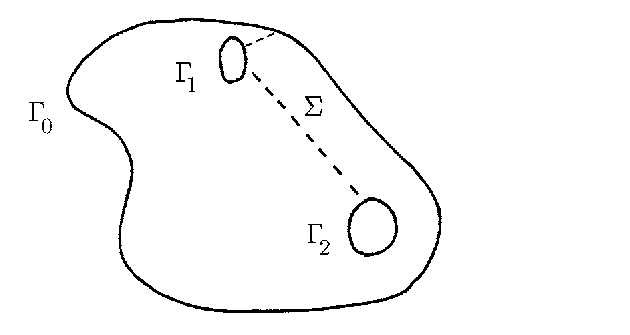
\includegraphics[width=0.42\textwidth]{figures/chapter01-figure02.png}
\caption{}
\label{fig:ch1-multiply-connected-domain}
\end{figure}

若 $\Omega$ 单连通, 则由 \eqref{eq:ch1-reduced-stokes-divergence}, 存在函数 $\rho$, 使
\begin{equation}
w=(D_2\rho,-D_1\rho).
\label{eq:ch1-stream-function-representation}
\end{equation}
条件 \eqref{eq:ch1-reduced-stokes-boundary} 等价于 $\rho=\partial\rho/\partial\nu=0$ 在 $\Gamma$ 上成立; 对 \eqref{eq:ch1-reduced-stokes-momentum} 微分后得到
\[
-\nu\Delta(D_2w_1-D_1w_2)=D_2f'_1-D_1f'_2.
\]
于是
\begin{equation}
\nu\Delta^2\rho=D_1f'_2-D_2f'_1
\in W^{m-1,\alpha}(\Omega),
\label{eq:ch1-biharmonic-equation}
\end{equation}
\begin{equation}
\rho=0,\qquad\frac{\partial\rho}{\partial\nu}=0
\quad\text{在 }\Gamma\text{ 上}.
\label{eq:ch1-biharmonic-boundary}
\end{equation}
双调和问题 \eqref{eq:ch1-biharmonic-equation}--\eqref{eq:ch1-biharmonic-boundary} 有唯一解 $\rho\in W^{m+3,\alpha}(\Omega)$, 由 \eqref{eq:ch1-stream-function-representation} 定义的 $w$ 是 \eqref{eq:ch1-reduced-stokes-momentum}--\eqref{eq:ch1-reduced-stokes-boundary} 的解, 且属于 $\mathbf W^{m+2,\alpha}(\Omega)$.

若 $\Omega$ 非单连通, 条件 \eqref{eq:ch1-reduced-stokes-divergence} 使我们能局部得到 \eqref{eq:ch1-stream-function-representation}, 即 $\rho$ 可能不是单值函数. 利用 \eqref{eq:ch1-reduced-stokes-boundary} 的进一步论证将在下一引理中给出; 它表明 $\rho$ 必为单值函数, 且
\begin{equation}
\rho=0\quad\text{在 }\Gamma_0\text{ 上},
\qquad
\rho=\text{常数}\quad\text{在 }\Gamma_i\text{ 上},\quad i=1,2,\ldots,
\label{eq:ch1-stream-function-component-values}
\end{equation}
\begin{equation}
\frac{\partial\rho}{\partial\nu}=0\quad\text{在 }\Gamma\text{ 上},
\label{eq:ch1-stream-function-normal-boundary}
\end{equation}
其中 $\Gamma=\Gamma_0\cup\Gamma_1\cup\Gamma_2\cup\cdots$ 是 $\partial\Omega$ 的连通分支分解; $\Gamma_0$ 是其中一个分支(例如, 当 $\Omega$ 有界时取其外边界), $\Gamma_1,\Gamma_2,\ldots$ 是其余分支.

这样, 关于 $\rho$ 的问题 \eqref{eq:ch1-reduced-stokes-momentum}--\eqref{eq:ch1-reduced-stokes-boundary} 化为方程 \eqref{eq:ch1-biharmonic-equation} 及边界条件 \eqref{eq:ch1-stream-function-component-values}--\eqref{eq:ch1-stream-function-normal-boundary}. 与前面相同, 该双调和问题有唯一解 $\rho\in W^{m+3,\alpha}(\Omega)$, 由 \eqref{eq:ch1-stream-function-representation} 定义的 $w$ 是 \eqref{eq:ch1-reduced-stokes-momentum}--\eqref{eq:ch1-reduced-stokes-boundary} 的解, 且属于 $\mathbf W^{m+2,\alpha}(\Omega)$.
\end{Proof}

\MBSourceStatementNumber{lemma}{5}
\begin{Lemma}
\label{lem:ch1-stream-function-single-valued}
设 $\Omega$ 是 $\mathbb R^2$ 中的开集, $w\in\mathbf W_0^{1,1}(\Omega)$ 是无散向量函数. 则存在唯一的单值函数 $\rho\in W^{2,1}(\Omega)$(流函数), 它满足 \eqref{eq:ch1-stream-function-component-values}, \eqref{eq:ch1-stream-function-normal-boundary} 以及
\begin{equation}
w=(D_2\rho,-D_1\rho).
\label{eq:ch1-stream-function-lemma-representation}
\end{equation}
\end{Lemma}

\begin{Proof}
先对光滑函数 $w$ 证明该结论. 对一般向量函数 $w$, 结论可由稠密性论证推广得到.

以 $\Gamma_0,\Gamma_1,\Gamma_2,\ldots$ 表示 $\Gamma=\partial\Omega$ 的各连通分支, 在 $\Omega$ 中作若干光滑割线 $\Sigma$, 使 $\Omega=\Sigma\cup\dot\Omega$, 其中 $\dot\Omega$ 是单连通开集. 对给定的光滑函数 $w$, 存在函数 $\rho$, 使 \eqref{eq:ch1-stream-function-lemma-representation} 在 $\dot\Omega$ 中成立. 显然 $\rho$ 在 $\overline\Omega$ 中光滑; 由于 $w=0$ 在 $\partial\Omega$ 上成立, $\operatorname{grad}\rho$ 在 $\partial\Omega$ 上为零, 因而 $\rho$ 在每个 $\Gamma_i$ 上为常数, 且 $\partial\rho/\partial\nu$ 在 $\partial\Omega$ 上为零. 通过在 $\Gamma_0$ 上指定 $\rho$ 的值使其唯一: $\rho=0$ 在 $\Gamma_0$ 上.

令 $\rho_\pm$ 表示 $\rho$ 在 $\Sigma$ 两侧 $\Sigma_+$ 和 $\Sigma_-$ 上的值. 对任意 $w$, 两侧的值本可不同; 但若 $w$ 在 $\partial\Omega$ 上为零且 $\rho$ 在每个 $\Gamma_i$ 上为常数, 它们必相同. 若 $M_\pm,P_\pm$ 是 $\Sigma_\pm$ 上两点且 $M_\pm\in\partial\Omega$, 则
\[
\rho(P_+)-\rho(M_+)
=\int_{\Sigma(M_+\to P_+)}w\,dx
=\int_{\Sigma(M_-\to P_-)}w\,dx
=\rho(P_-)-\rho(M_-).
\]
又因 $\rho(M_+)=\rho(M_-)$, 得 $\rho(P_+)=\rho(P_-)$ 在 $\Sigma$ 上成立.
\end{Proof}

\subsection{Stokes 问题的特征函数}
\label{subsec:ch1-stokes-eigenfunctions}

设 $\Omega$ 是 $\mathbb R^n$ 中任意有界开集. 定理 \ref{thm:ch1-stokes-existence-uniqueness} 所定义的映射
\[
\Lambda:f\longmapsto\frac1\nu u
\]
显然是从 $\mathbf L^2(\Omega)$ 到 $V$, 进而到 $\mathbf H_0^1(\Omega)$ 的连续线性映射. 因为 $\Omega$ 有界, $\mathbf H_0^1(\Omega)$ 到 $\mathbf L^2(\Omega)$ 的自然嵌入紧\setcounter{footnote}{0}\footnote{Sobolev 空间中的紧性定理将在 \MBUnresolvedReference{chapter-section}{Chapter 2, \S1} 回顾.}, 故把 $\Lambda$ 看作 $\mathbf L^2(\Omega)$ 中的线性算子时, 它是紧算子. 该算子还是自伴的, 因为
\[
(\Lambda f_1,f_2)=\nu((u_1,u_2))=(f_1,\Lambda f_2),
\]
其中 $\Lambda f_i=u_i$, $i=1,2$.

因此, 算子 $\Lambda$ 有一个由特征函数 $w_j$ 构成的标准正交序列:
\[
\Lambda w_j=\lambda_jw_j,\qquad j\geq1,
\qquad\lambda_j>0,\quad\lambda_j\to+\infty\ (j\to+\infty),
\]
并且
\begin{equation}
w_j\in V,\qquad
((w_j,v))=\lambda_j(w_j,v),\qquad\forall v\in V.
\label{eq:ch1-stokes-eigenproblem}
\end{equation}
通常有
\begin{equation}
\begin{aligned}
(w_j,w_k)&=\delta_{jk},\\
((w_j,w_k))&=\lambda_j\delta_{jk},\qquad\forall j,k.
\end{aligned}
\label{eq:ch1-stokes-eigenfunction-orthogonality}
\end{equation}
再次利用定理 \ref{thm:ch1-stokes-existence-uniqueness}, 可如下解释 \eqref{eq:ch1-stokes-eigenproblem}: 对每个 $j$, 存在 $p_j\in L^2_{\mathrm{loc}}(\Omega)$, 使
\[
-\nu\Delta w_j+\operatorname{grad}p_j=\lambda_jw_j
\quad\text{在 }\Omega\text{ 中},
\]
\[
\operatorname{div}w_j=0\quad\text{在 }\Omega\text{ 中},
\qquad
\gamma_0w_j=0\quad\text{在 }\Gamma\text{ 上}.
\]
若 $\Omega$ 是 Lipschitz 集, 由命题 \ref{prop:ch1-gradient-regularity}, $p_j\in L^2(\Omega)$. 若 $\Omega$ 是 $C^m$ 类集合($m$ 是不小于 $2$ 的整数), 反复应用命题 \ref{prop:ch1-stokes-regularity-apriori} 得
\begin{equation}
w_j\in\mathbf H^m(\Omega),\qquad
p_j\in H^{m-1}(\Omega),\qquad\forall j\geq1.
\label{eq:ch1-stokes-eigenfunction-finite-regularity}
\end{equation}
若 $\Omega$ 是 $C^\infty$ 类集合, 则由 \eqref{eq:ch1-stokes-eigenfunction-orthogonality},
\begin{equation}
w_j\in\mathbf C^\infty(\overline\Omega),\qquad
p_j\in C^\infty(\overline\Omega),\qquad\forall j\geq1.
\label{eq:ch1-stokes-eigenfunction-smoothness}
\end{equation}
$\lambda_j$ 在 $j\to\infty$ 时的行为已知, 即
\begin{equation}
\lambda_j\sim c j^{n/2}.
\label{eq:ch1-stokes-eigenvalue-asymptotic}
\end{equation}
其中 $c$ 是适当的常数, $n$ 是空间维数(见 G. Métivier [1]). 注意, 这一行为与带有 Dirichlet 或 Neumann 边界条件的 Laplace 算子的特征值行为相同; 关于这些经典结果, 例如见 R. Courant 和 D. Hilbert, \emph{Methods of Mathematical Physics}, Publishers, Inc., New York, 1953.
